%%%%%%%%%%%%%%%%%%%%%%%%%%%%%%%
%%Derived from "Metropolis" (beamerthememetropolis)
%
% May need to run 
% 1) LaTex -> PDF
% 2) LaTex -> DVI -> PDF
% 3) LaTex -> DVI -> PS -> PDF
% 4) XeTex -> PDF
%
%%%%%%%%%%%%%%%%%%%%%%%%%%%%%%%%%%%%%%



%%%%%%%%%%%%%%%%%%%
% BEAMER CHOICES
%%%%%%%%%%%%%%%%%%%

\documentclass{beamer}
\mode<presentation>{\usetheme{metropolis}}

% Define your custom hex color (use UPPERCASE letters for the hex code)
\definecolor{MyHexColor}{HTML}{276221}
\setbeamercolor{frametitle}{bg=MyHexColor, fg=white}

%%%%%%%%%%%
% PACKAGES
%%%%%%%%%%%

\usepackage[english]{babel}
\usepackage{times}
\usepackage[T1]{fontenc}

\usepackage{comment}
\usepackage{amsmath}
\usepackage{amsthm}                           % Required for theorem environments
\usepackage{bm}                               % Required for bold math symbols (used in the footer of the slides)
\usepackage{graphicx}                         % Required for including images in figures
\usepackage{booktabs}                         % Required for horizontal rules in tables
\usepackage{multicol}                         % Required for creating multiple columns in slides
\setlength{\columnsep}{0.1mm}


\usepackage{microtype}                        % Better typography
%\usepackage{tocstyle}                         % Required for customizing the table of contents
\usepackage{caption}
\captionsetup{labelformat=empty,labelsep=none}
\usepackage{mathtools}
\usepackage{subcaption}
\usepackage{nicefrac}
\usepackage{csquotes}

\usepackage{enumitem}	                        %spread enumeration over multiple slides
\usepackage{pdfpages}
\usepackage{tikz}  
\usepackage[absolute, overlay]{textpos}      %position textblocks (absolute) on the page
\setlength{\TPHorizModule}{\textwidth}
\setlength{\TPVertModule}{\textwidth}


\usepackage{appendixnumberbeamer}
\usepackage{booktabs}
\usepackage{xspace}
 \newcommand{\themename}{\textbf{\textsc{metropolis}}\xspace}



%%%%%%%%%%%%%%%%%%%%%%%%%%%%%%%
% TITLE PAGE AND BEAMER OPTIONS
%%%%%%%%%%%%%%%%%%%%%%%%%%%%%%%%

\title{Sustainability Now! \\
Sustainability Concepts and Frameworks \\
Lecture 01}
%\subtitle{(or why common sense makes sense) }
\date{\today}
\author{Bruce D. Marron}
%\institute{UTECA}
\titlegraphic{
\begin{tikzpicture}[overlay]
%  \node[anchor=south west] at (0,-8.5) {
\includegraphics[scale= 0.35]{graphics/UMA_Logo.png}};
  \node[anchor=south west] at (0,-8.5) {
\includegraphics[scale= 0.35]{graphics/UTECA_Logo.png}};
 \end{tikzpicture}
 }

%---------------OPTIONALS-------------------------------------------------------
% (optional, use only with lots of authors)
%\author[Author, Another] {F.~Author\inst{1} \and S.~Another\inst{2}}

% \institute[Universities of Somewhere and Elsewhere] 
% {  \inst{1}%
%  Department of Computer Science\\
%  University of Somewhere
%  \and
%  \inst{2}%
%  Department of Theoretical Philosophy\\
%  University of Elsewhere
%  }

% (optional, should be abbreviation of conference name)
%\date[CFP 2003] {Conference on Fabulous Presentations, 2003}

% This is only inserted into the PDF information catalog. Can be left out. 
%\subject{Theoretical Computer Science}


% the table of contents pops up at the beginning of each subsection
%\AtBeginSubsection[]                                     
% {
%  \begin{frame}<beamer>{Outline}
%    \tableofcontents[currentsection,currentsubsection]
%  \end{frame}
% }


% uncover everything in a step-wise fashion
%\beamerdefaultoverlayspecification{<+->}              
%-----------------------------------------------------------------------------------------------------


%%%%%%%%%%%%%%%%%%%%%%%%%
% SPECIALTY NEW COMMANDS
%%%%%%%%%%%%%%%%%%%%%%%%%%
 
% Arrow over vector
\newcommand{\amsvect}{%
  \mathpalette {\overarrow@\vectfill@}}
\def\vectfill@{\arrowfill@\relbar\relbar{\raisebox{-3.81pt}[\p@][\p@]{$\mathord\mathchar"017E$}}}


% Nice-looking fractions
\newcommand\ddfrac[2]{\frac{\displaystyle #1}{\displaystyle #2}}





%#############
%  DOCUMENT
%#############


\begin{document}


%%%%%% TITLE PAGE %%%%%%%%%%%%
\begin{frame}
  \titlepage
\end{frame}


%%%%%%%%%%%%%%%%%%%%
% SLIDES
%%%%%%%%%%%%%%%%%%%%

% tikzpics
%  anchor=south west] at (3.0,-4.5) ==> 3 to the right; 4.5 down from the top


%%%%%%%%%%%%%%%%%%%%%%%%%%%%%
\section{Sustainability?}
%%%%%%%%%%%%%%%%%%%%%%%%%%%%%

%Slide-------------------------------------------------------------------
\begin{frame}{Sustainability}
\vspace{-10 mm}
\large {\textbf{Sustainability:} Concepts and frameworks of stewardship, which are translated to direct human behaviors (decisions and management actions) and applied across multiple, interlinked complex adaptive systems (CAS), to ensure intergenerational equity.\\
\vspace{5 mm}
\textbf{The Goal:} Flourishing of the Seven Generations.}\\
\vspace{5 mm}
\begin{tikzpicture}[overlay]
  \node[anchor=south west] at (2.5,-2.8) {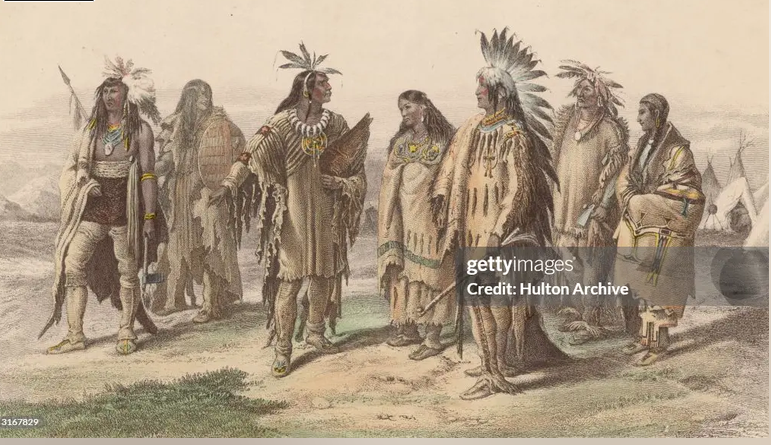
\includegraphics[scale=.2]{graphics/Iriquois.png}};  
 \end{tikzpicture}


\end{frame}


%Slide-------------------------------------------------------------------
\begin{frame}{Sustainability}


\begin{tikzpicture}[overlay]
  \node[anchor=south west] at (3.0,-4.3) {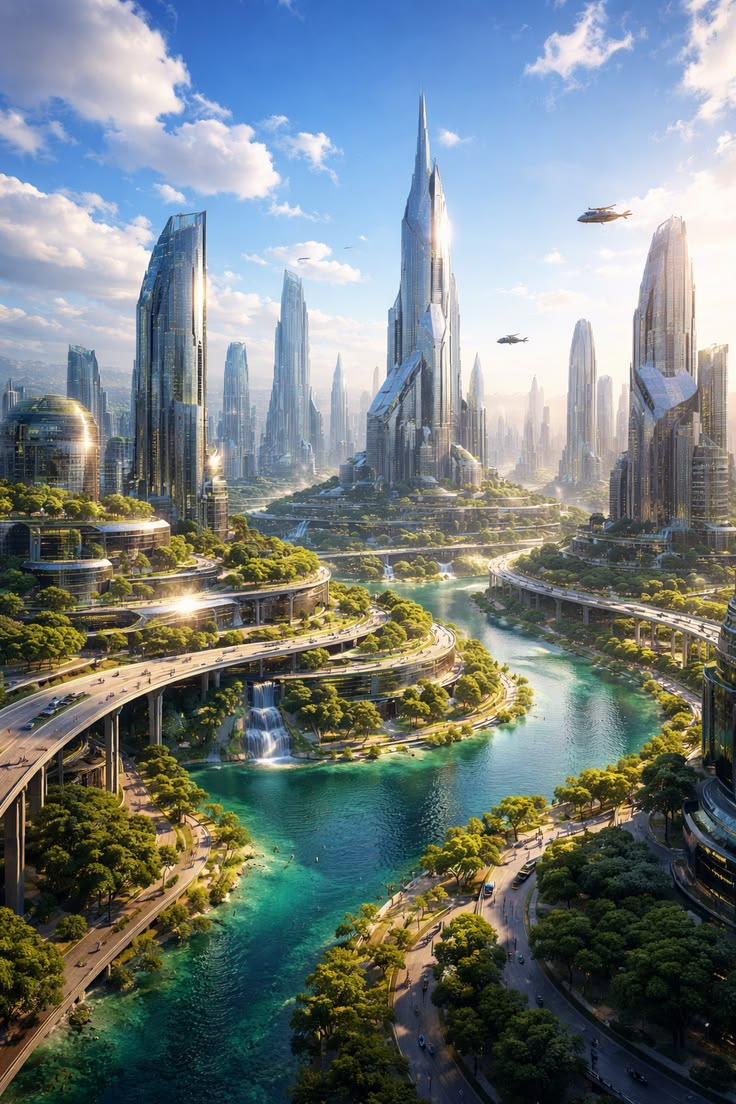
\includegraphics[scale=.2]{graphics/DreamCity.jpeg}};  
 \end{tikzpicture}


\end{frame}


%Slide-------------------------------------------------------------------
\begin{frame}{Sustainability}
\vspace{-40 mm}
Gro Harlem Brundtland, 41 \\
First Woman Prime Minister of Norway, 1981

\begin{tikzpicture}[overlay]
  \node[anchor=south west] at (8.0,-1.8) {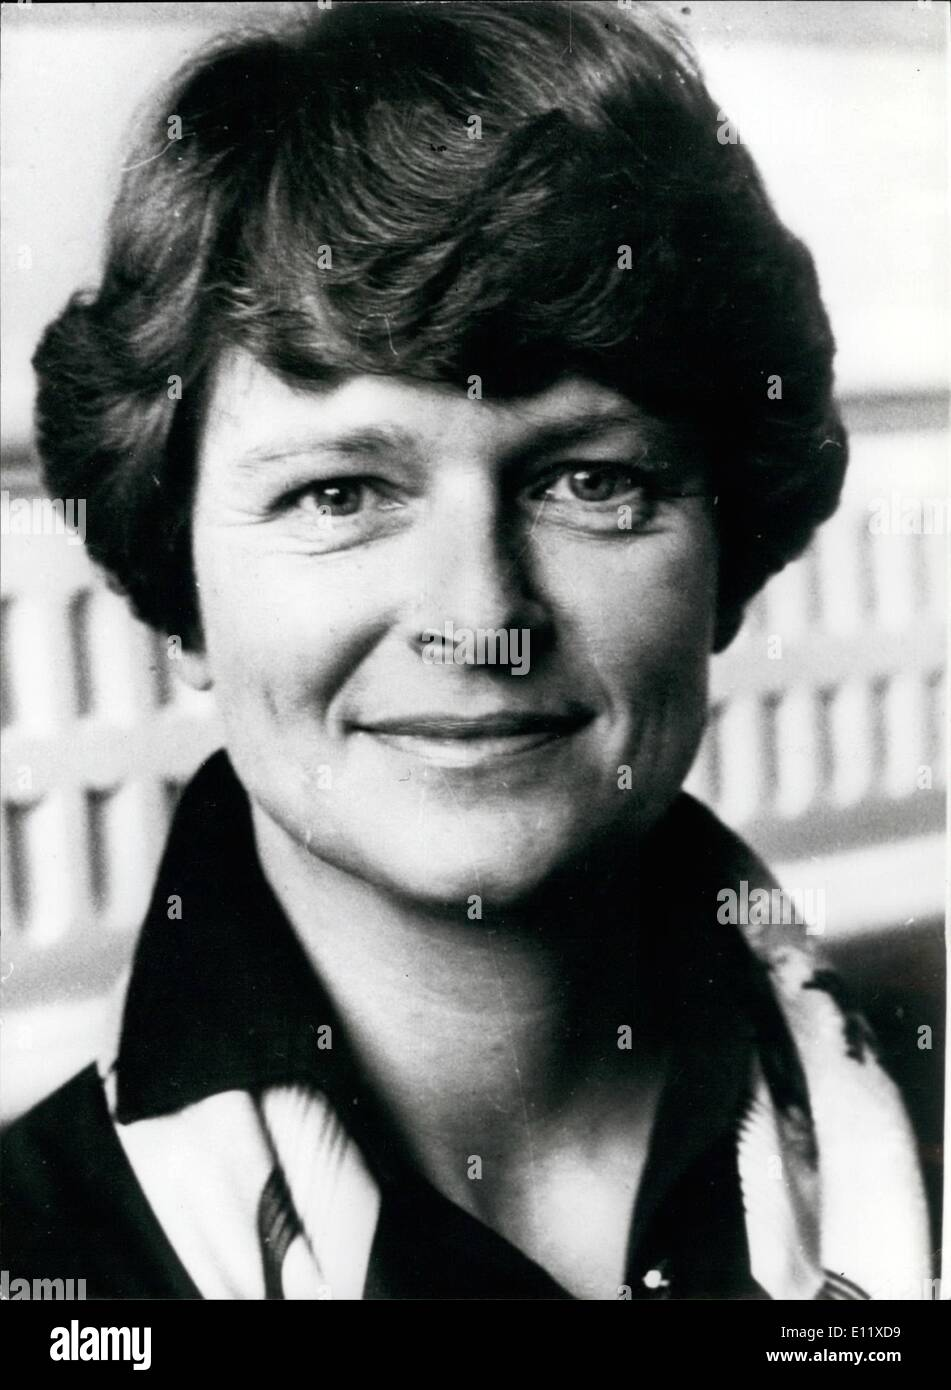
\includegraphics[scale=.3]{graphics/GHBrundtland.jpg}};  
 \end{tikzpicture}
 
 \begin{tikzpicture}[overlay]
  \node[anchor=south west] at (-1.0,-2.0) {
\includegraphics[scale=.17]{graphics/BrundtlandReport.png}};  
 \end{tikzpicture}
 
 
 \begin{tikzpicture}[overlay]
  \node[anchor=south west] at (0.2,-3.0) {\textit{"...development that meets the needs of the present without}};
  \node[anchor=south west] at (0.2,-3.5) {\textit{compromising the ability of future generations}};
  \node[anchor=south west] at (0.2,-4.0) {\textit{to meet their own needs"}};
 \end{tikzpicture}
 

 \end{frame}


%Slide-------------------------------------------------------------------
\begin{frame}{Complex Adaptive Systems}

\begin{tikzpicture}[overlay]
  \node[anchor=south west] at (0.5,-3.5) {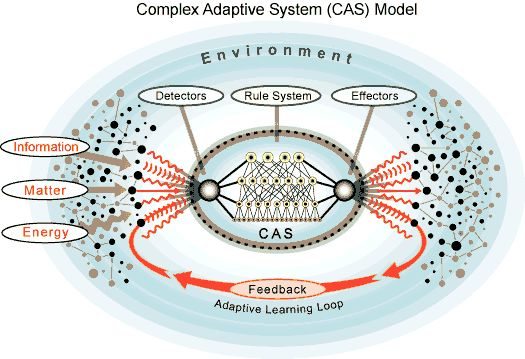
\includegraphics[scale=.5]{graphics/CAS1.jpeg}};  
 \end{tikzpicture}


\end{frame}

%Slide-------------------------------------------------------------------
\begin{frame}{Complex Adaptive Systems}
\vspace{-15 mm}

{\large \textbf{Complex} means}...\\
{\large \textbf{Adaptive} means} ...\\
{\large \textbf{System} means} ...\\

\vspace{10 mm}

\begin{large}
...Emergence... \\
\hspace{15 mm}...Self-Organization... \\
\hspace{30 mm}...Feedback Loops... \\
\hspace{45 mm}...Resilience...
\end{large}

\end{frame}


%Slide-------------------------------------------------------------------
\begin{frame}{Complex Adaptive Systems}

\begin{tikzpicture}[overlay]
  \node[anchor=south west] at (1.5,-3.5) {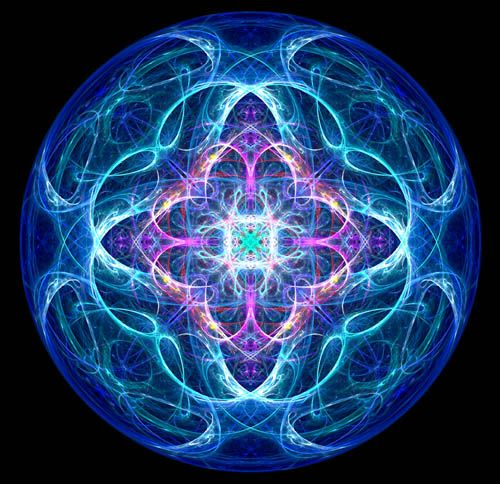
\includegraphics[scale=.4]{graphics/Fractal_CAS.jpeg}};  
 \end{tikzpicture}

\end{frame}


%Slide-------------------------------------------------------------------
\begin{frame}{Complex Adaptive Systems}

\begin{tikzpicture}[overlay]
  \node[anchor=south west] at (0.6,-3.5) {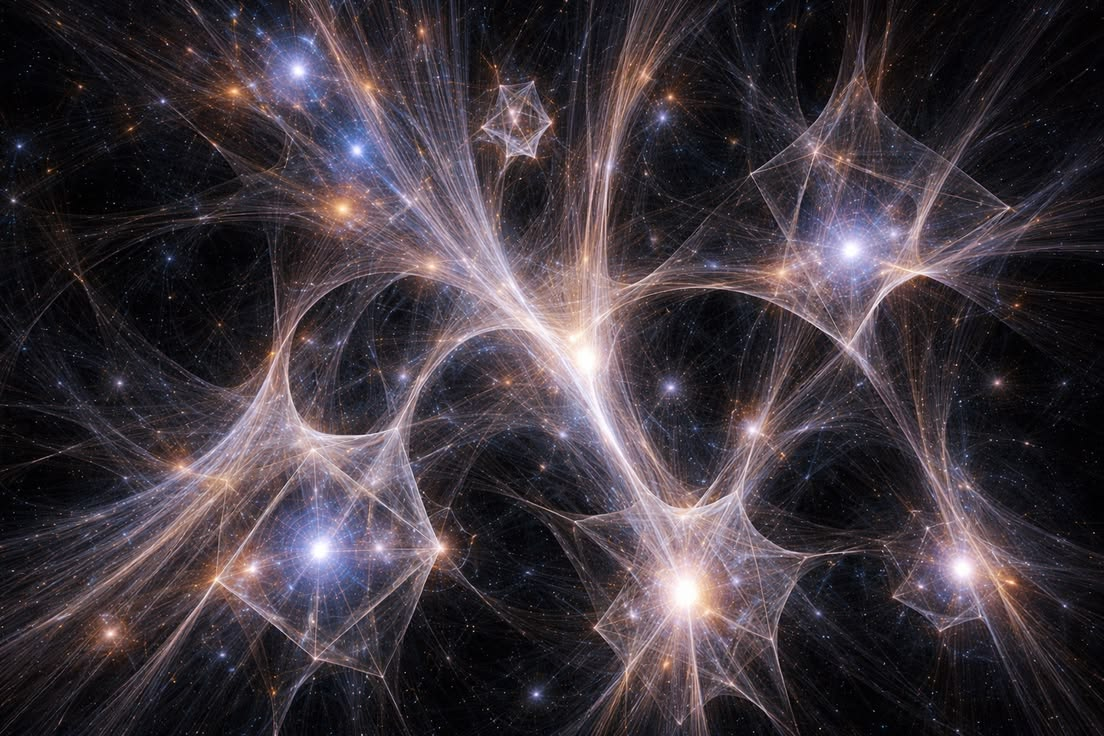
\includegraphics[scale=.25]{graphics/Fractal_CAS2.jpeg}};  
 \end{tikzpicture}

\end{frame}





%Slide-------------------------------------------------------------------
\begin{frame}{Resilience}
\large {Resilience is the use of dynamic human imagination to adapt, transform, evolve, innovate, self-organize, restructure, and survive when confronted with identity-level disruptive change from turbulence, emergence, collapse, devastation, or crisis} \\
\vspace{5 mm}
\large {Reslience pathways may lead to adaptation (The Ship of Theseus) or transformation (Death of the Gold Standard)}\\ 
\vspace{5 mm}
\large {Resilience pathways may lead to dead ends}\\
\vspace{6 mm}
\large \textit{"Sometimes you need to break the resilience of the current system to enable shifts away from the current pathway(s) into new ones, into alternative basins of attraction"}

\end{frame}




%%%%%%%%%%%%%%%%%%
%END OF DOC
%%%%%%%%%%%%%%%%%
\end{document}
